
%\chapter{The effect of phenotypic plasticity on plant community dynamics}
%Hypothesis on the cumulative effect on niche and interactions.
%
%\section{Individual resistance and resilience against drought events}
%Amplitude and length of the event :\\
%- severity effect reduced by lower tau ?\\
%- resistance versus resilience: H0: conservative strategy have higher resistance, H1 : low tau allows for re-equilibrium and increase resistance (low amplitude and long length. H2: high tau allow to avoid dead-end situation during short severe drought (high resilience)
%\section{Community response to drought event}
%coexistence effect vs resistance/resilience effect\\
%uniform vs heterogenous (plasticity wise) community response
%H1: 
%

\begin{fullwidth}
This second result chapter examines the effects of phenotypic plasticity at the scale of the community. Another parameter filtering processes is performed and described in the first section of this chapter. The second part focuses of the effects of plasticity of the main properties of the community. The impact of plasticity on species diversity is particularly investigated. This chapter gives a glimpse of the potential of the model to answer various questions around the role of intraspecific variations on diverse community properties.
\end{fullwidth}

\chapter{Community level simulations: non plastic community}


\section{Parameter filtering}
\subsection{Method}

%\paragraph{Field data}
%Field data has been collected between years 201 .. and 201 by Claire Deleglise and al. (). Not used here.

\paragraph{Weather data}
Weather data for the time period between 1959 and 2014 has be computed by the MeteoFrance model SAFRAN by ... using GPS coordinates, slope, azimuth and horizon computed from a digital elevation model. These parameters were also used by the model CROCUS to compute snow accumulation and snow melting. These high frequency data (resolution under 1h) have been averaged on a daily time-step and used to compute input variables for \model. The snow in particular defines the length of the growing season starting with the first snow melt of the year and finishing the day of the first snow fall of autumn or winter.

The simulated years above 2014 are randomly sampled form the existing dataset between 1995 and 2014.

\paragraph{Parameter filtering}
Community level parameter filtering is conduced for a new table of parameter sets. These parameter sets are ... from accepted parameters and joined with LHS random sampling for five community level parameters: seed germination density, drought mortality, ageing mortality, plasticity cost for environmental sensing and plasticity cost for trait changes (see chapter \ref{chapter:model-description} for details).

Few words on why plasticity cost parameters: time limits, distinguish the benefit of plasticity itself, not combined effect. Should have done simulations with no cost to have an idea of plasticity cost effect. 

The simulations run over 300 hundreds years for 6 sites described in table \ref{table:sites} on squares of ... square centimetres. The simulation is stopped and the parameter set rejected if no individual persist and the seedbank is empty. The seedrain is composed of seeds contained in the seedbank and seeds from the metacommunity. The total of seeds is defined by the seed germination density and the area simulated. The seeds from the simulated community represent up to 80 \% of the seedrain, less if the seed production is limiting. The first ... years are not taken into account in the filtering process to let the community settle.


\paragraph{Simulations}

\subsection{Results}

Simulations done. Need to illustrate the results.\\

\paragraph{Effect of parameters}
On stability and on diversity (functional and species)\\
Random forest approaches like sensitivity analysis at individual scale.


\section{Non plastic communities}
Trade-off, diversity, stability ...


\paragraph{Ecological trade-off ?}
Is there a selection of some parameters ? Are there ecological trade-off (resource use strategy and reproduction) emerging from the model ?

\chapter{Plasticity: impact on species fitness and diversity}

Plasticity in integrated framework and full community simulations. Plasticity mechanisms, but also plasticity as a strategy (look at the cost and tau). 

Effects on productivity and coexistence. Difference in the correlation ?

Effect of tau on persistence.

\section{Plasticity and diversity}

Now 

\subsection{Method}

\paragraph{Simulations}
To test the effect of plasticity on coexistence and community dynamics, runs from the parameter filtering are used as starting points to limit the simulation time of the stabilisation phase. For each parameter set tested, 6 different sites were tested during the calibration phases, 77 parameter sets were accepted and a sample of ... were tested, resulting in ... communities. Each of those is the starting point of three parallel runs that differ only by the allocation algorithm used: \textit{non plastic}, \textit{fixed-equilibrium} and \textit{plastic-optimisation}. The \textit{fixed-equilibrium} is favoured to \textit{fixed-optimisation} algorithm because previous part of the document focused on this algorithm and because it is simpler to analyse. The \textit{plastic-optimisation} algorithm is still simulated, despite the relatively poor performance results observed in constant conditions and the high convergence, because the introduction of plasticity cost, continuous species specific plasticity ($0 < \tau < 1$), and temporal and spatial heterogeneity should mitigate the negative sides of this allocation mechanism and give information of processes at stake.

The plasticity costs (maintenance: related to the value of $\tau$, and displacement: relative to changes in phenotypes) defined in the parameter sets are applied to all algorithms. In \textit{non plastic} simulations, this results in artificial additional costs to species with low values of $\tau$ but with no potential gain from plasticity as the allocation is non plastic. 


\paragraph{Statistical tests}

The differences of effects between the different types of plasticity on the variables of interest are computed unpaired Wilcoxon tests assuming an independence of the the different data points. This assumption of statistical independence is justified by the normalisation for each parameter set of the variables relative to the mean of the \textit{non plastic} group. This normalisation allows to compare the simulations between the parameters sets. The interactions and other level (site, and autocorrelations) are discussed later in this section. 

The normalisation $Vn_{a, p, t, s}$ of the variable $V$ for the allocation algorithm $a$, the parameter set $p$, the time $t$ and the site $s$ is given by the following formula:

\begin{align}
Vn_{a, p, t, s} &= \frac{V_{a, p, t, s}}{ \bar{V} }\\
\bar{V} &= \frac{\sum_{a == \text{\textit{non plastic}}}{} Vn_{p, t, s} }{n}
\end{align}

where $n$ is the number of observations for the \textit{non plastic} algorithm.

\subsection{Results}

%Need to run the simulations. Script is almost ready, parameters are filtered from previous step.
%
%\paragraph{General behaviour} ?
%gradient along climatic gradient ? did I save the climate ? Nope, can't really say anything about it.

\paragraph{Effect on coexistence}

The level of coexistence is evaluated by the number of distinct species that manage to maintain at least one individual or produce at least one seed at the end of the season. This criterion allow to ignore the potential non stable diversity introduced by the "meta-community invasion" (sampling of species in the meta-community pool) and to consider species that can be filtered out sue to seed mortality. The number of species increases in almost all simulated years and sites for both plastic allocation algorithms, with a median of 1.5 times the number of species in \textit{non plastic} simulations (see figure \ref{fig:species_richness}). This factor can go up to 6 for \textit{fixed-equilibrium} and 9 for \textit{plastic optimisation}.


\begin{marginfigure}\label{fig:species_richness}
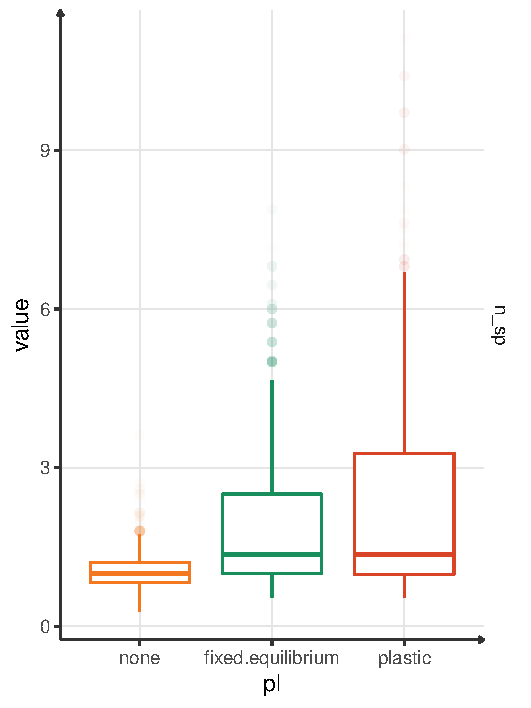
\includegraphics[]{./2_PP/Figures/Comm/comm_n_sp_differences.pdf}
\caption[Relative species richness in plasticity treatments]{Relative species richness in the three plasticity treatment. To negate the variability due to the parameter sets, the realised number of species is divided by the median number of species in \textit{non plastic} treatment for each parameter set. The variability is due to random invasion and climatic variability (inter-sites and inter-seasons).}
\end{marginfigure}

The effect of plasticity on coexistence is driven by the benefits of plasticity at the individual scale. These benefits are mitigated by the cost of plasticity, particularly the maintenance cost that affect all species relatively to their potential plasticity.

%Plasticity is responsible for high portion of variability, but also parameters: plasticity cost parameters:

\begin{figure}%[tb]
%    \classiccaptionstyle
%\sidebysidecaption{0.60\textwidth}{0.3\textwidth}{%
    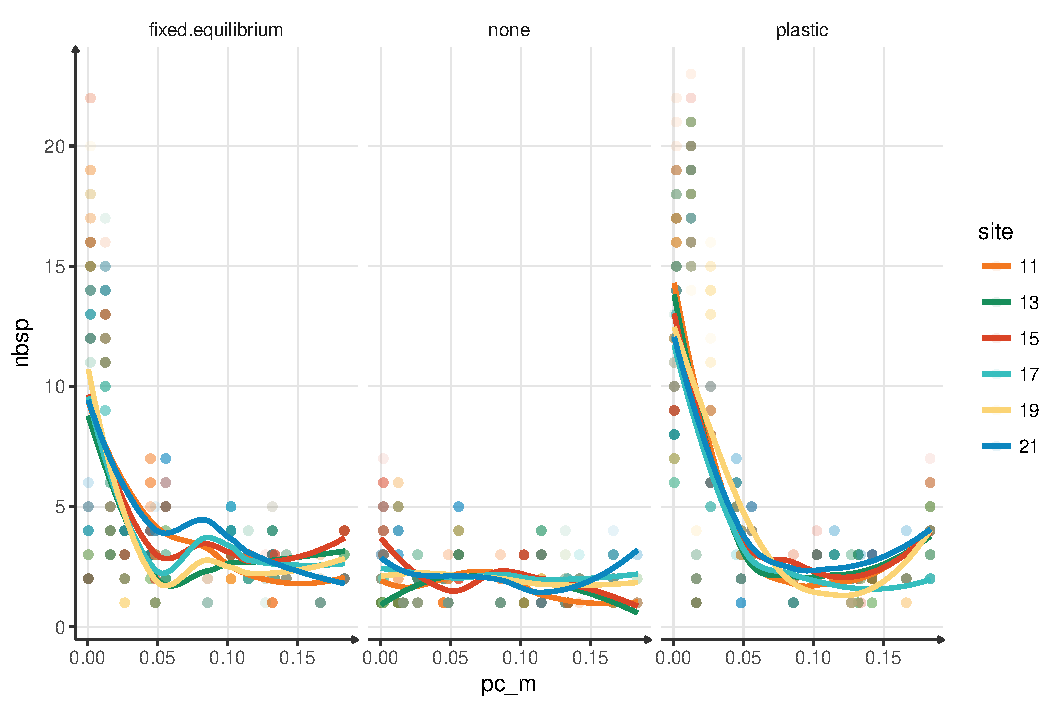
\includegraphics[width=1\linewidth]{./2_PP/Figures/Comm/comm_n_sp_pc_m.pdf}%
%}{%
  \caption[Maintenance plasticity cost effect on species richness]{Effect of the cost of plasticity-maintenance on the absolute number of species in the three plasticity treatments. Individual season values (points) and site-specific trends (gam smoothing line) are represented.}
  \label{fg:pl_cost}
%  }
\end{figure}

Low values of plasticity maintenance cost (see figure \ref{fig:pl_cost}) show higher diversity for both plastic allocation algorithms. This trend is consistent across sites despites some inter-annual variability in the diversity. The effect is a bit less stronger for \textit{fixed-equilibrium} than for \textit{plastic-optimisation} (as already observed in figure \ref{fig:species_richness}).

%Consistent trends between sites. Inter-season variability (why didn't I save the weather?). Not super clean. Similar (but lower start) for plastic distance diversity. Can be because of interactions %or because non variable enough.

%Why higher diversity: it is not because of higher density (number of individual per m2).
%But changes in filtering: more species

The mechanisms through which the phenotypic plasticity impacts species richness are multiple (refer to the figure \ref{fig:plasticity-effect} in chapter \ref{part:literature}). However it is hard to disentangle them all.

The density can be affected by the phenotypic plasticity leading to higher species diversity\cite{lepik_high_2005}, higher density leading to the sampling of more species. The density, estimated by the number of individual after the reproduction phase (persisting individuals and produced seeds), is consistently higher in \textit{plastic} simulations, but the difference is relatively low (around 3\% higher than the \textit{non plastic} median density) and an order of magnitude lower than inter-annual and inter-site variations that can go up to 40\% difference relative to the median density (for any given parameter set).


\begin{marginfigure}\label{fig:tiller_density}
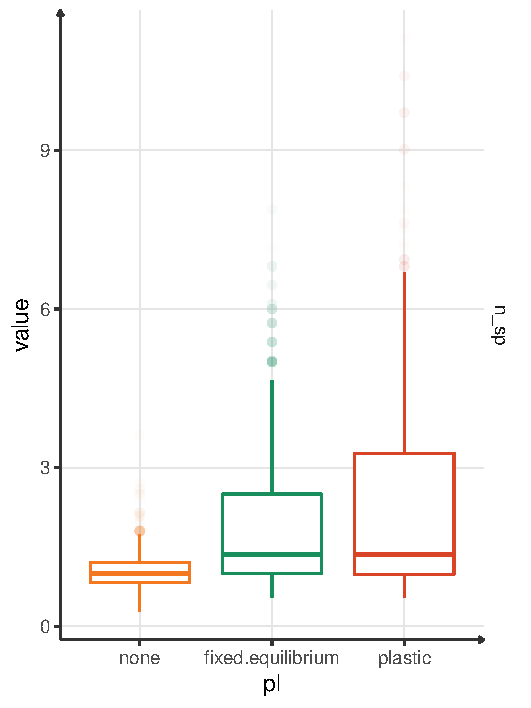
\includegraphics[]{./2_PP/Figures/Comm/comm_n_sp_differences.pdf}
\caption[Relative plant density in plasticity treatments]{Relative plant density in the three plasticity treatment. To negate the variability due to the parameter sets, the realised number of plant is divided by the mean number of plant in \textit{non plastic} treatment for each parameter set. The plant density is estimated with the output of the reproduction process.}
\end{marginfigure}

If the plant estimated density increases, the number of species relative to the plant density ... with plasticity.

\begin{figure}%[tb]
    \classiccaptionstyle
\sidebysidecaption{0.5\textwidth}{0.4\textwidth}{%
%    \includegraphics[width=1\linewidth]{./2_PP/Figures/Comm/comm_species_density.pdf}%
}{%
  \caption[Species richness relative to plant density]{Species richness relative to plant density for the three plasticity treatments.}
  \label{fg:species_per_plant}
  }
\end{figure}


%\paragraph{Plasticity selection}

%Not done yet. when is plasticity selected: is there a correlation between environment variables (or variations and plasticity selection). trade-off with other traits ?
\paragraph{Productivity}

Productivity is also susceptible to be impacted by the phenotypic plasticity at the community level. Multiple mechanisms can be involved, but in any case higher productivity is achieved by high efficiency in the resources given, and plasticity can affect this efficiency at individual level (with positive effects as observed in section \ref{chapter:individual}) or at the community scale with changes in the dominant species and competition intensity.

\begin{marginfigure}\label{fig:total_BM_comm}
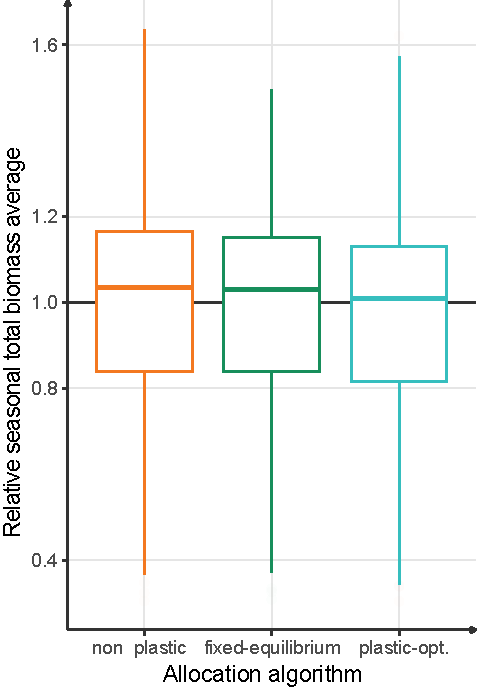
\includegraphics[width = \textwidth]{./2_PP/Figures/Comm/comm_BMtot_differences.pdf}
\caption[Average total biomass in plasticity treatments]{Average total biomass relative to \textit{non plastic} simulations, in the three plasticity treatments.}
\end{marginfigure}

The productivity of the \textit{non plastic}, \textit{fixed-equilibrium} and \textit{plastic-optimisation} allocation algorithm show little differences. The \textit{non plastic} simulations average biomass tend to be a bit higher in certain cases. Like the diversity and density, the normalised yearly average biomass does not show great variations between plasticity, but higher variability between sites and seasons. \textit{Non plastic} and \textit{fixed-equilibrium} median are quite similar, and the \textit{plastic-optimisation} show lower productivity than the other two algorithms.

%\paragraph{Community structure}
%
%Because changes in community structure, no changes in density or productivity but, changes in structure, and competition evenness.
%
%\begin{figure}%[tb]
%%    \classiccaptionstyle
%%\sidebysidecaption{0.60\textwidth}{0.3\textwidth}{%
%    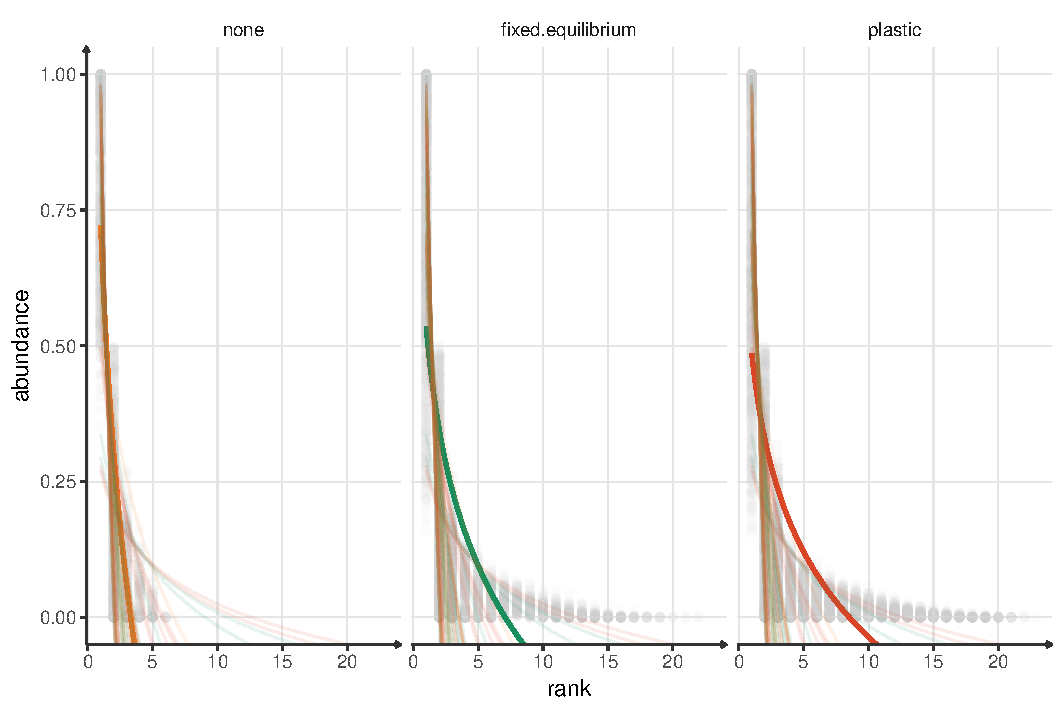
\includegraphics[width=1\linewidth]{./2_PP/Figures/Comm/comm_RAC_pl.pdf}%
%%}{%
%  \caption[Rank-Abundance curves fits]{Rank-Abundance curves.}
%  \label{fg:RAC}
%  %}
%\end{figure}



\paragraph{Plasticity: a winning strategy ?}

The allocation algorithm is expected to alter the fitness of potentially plastic plants. The selective effect of the allocation algorithms is investigated by plotting the $\tau$ value of species that are maintained in only one of the algorithms. Because of the plasticity cost, the selection of species with low values of $\tau$ signifies an improvement of the fitness due to plasticity. The distribution of $\tau$ is fairly high for \textit{non plastic} species and almost 75\% of the species have a value above 0.8, whereas \textit{fixed-equilibrium} specific species have lower values ranging from 0.2 to 1 with the median arond 0.7 and the \textit{plastic-optimisation} species have even lower values with a median around 0.55.
%Are plastic species more selected than the other ? Probably a bell-shape curves


\begin{marginfigure}\label{fig:tau}
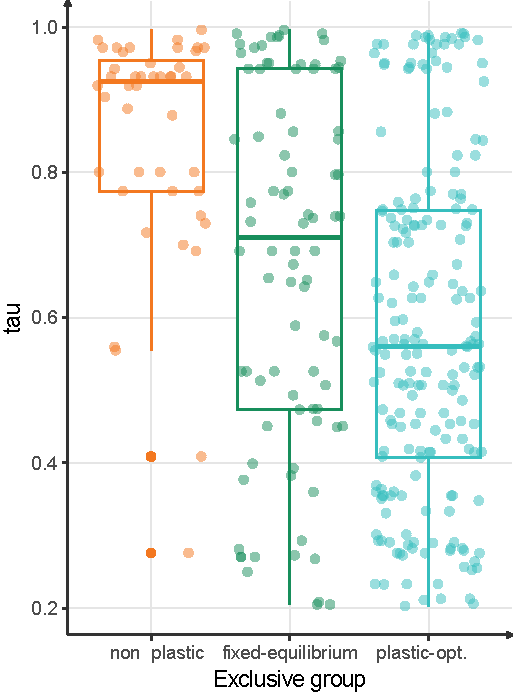
\includegraphics[]{./2_PP/Figures/Comm/comm_tau_differences_exclusive_groups.pdf}
\caption[Plasticity levels in exclusive groups]{Plasticity levels of species that are present in only one type of plastic treatment.}
\end{marginfigure}


%\section{Strategy}

%\subsection{Results}
\paragraph{Variable strats}

Select different strat? meh, from very site specific strats (one dominant species), to more variable within the site, but less differences between the strats. Shift from beta diversity to alpha diversity.

%Lead to changes in strats? If yes, is it direction\\
%al, or is the direction depends on species?%
%Do species change a lot there strategies?

%Is it always in the same direction for all species ? (reproduce Kichenin).

\paragraph{Different diversities}


\begin{figure}\label{fig:diversities}
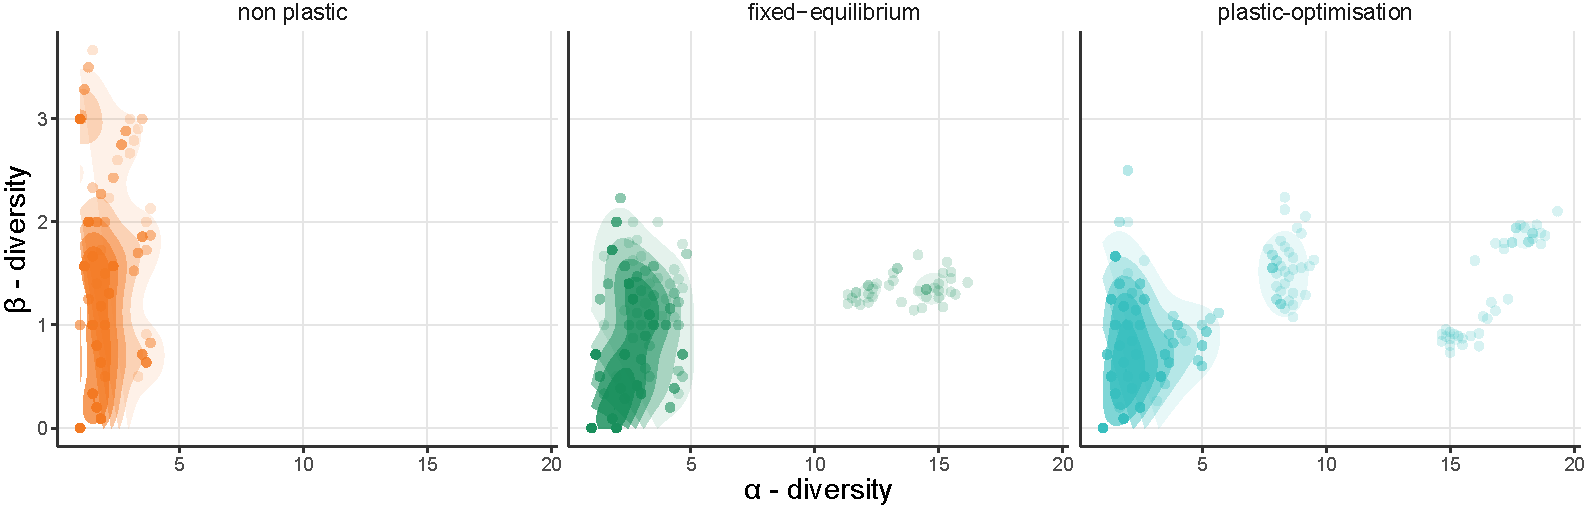
\includegraphics[]{./2_PP/Figures/Comm/comm_div_differences_alpha_beta.pdf}
\caption[Alpha and beta diversities as function of the allocation mechanism.]{Alpha and beta diversities as function of the allocation mechanism.}
\end{figure}

\subsection{Discussion}
\paragraph{Competition evenness}

Plasticity allows the emergence of new phenotypes that are plastic. Leading to higher density in competitors, and greater evenness. Hard to detect because not the same number of species, or require other experiments. 

\paragraph{shift in strategy}


also, Jung \cite{jung_intraspecific_2014} show contrasting response between species and within species - might not be the best 

\paragraph{Different mechanisms for different diversities}

%why higher alpha div

Plasticity allows for bigger niche (variability dimension), more chance to build enough "growth potential" to persist. Otherwise, other species that are dominant, because other species can settle, take advantage of it.
Should look at the growth rates hierarchy for a couple of simulations.

% but also lower beta


% What does it mean to modelling and to community properties ?



\paragraph{Independence of points}

Interaction between plasticity effects and parameter sets, but the interest here, even if  it is interesting. Higher variance due to site and weather. The almost perfect knowledge of models allows an extremely precise decomposition of the effects, but at the risks of loosing broad effects. The difficulty is to measure the relative strength of these effects, and generalise. But, by essence, the parameters are suspected to have a significant effect that can be identified, otherwise it would not have been included in the model.

\subsection{Phenotypic plasticity and global change}

climate 

management